\documentclass[conference]{IEEEtran}
\IEEEoverridecommandlockouts
% The preceding line is only needed to identify funding in the first footnote. If that is unneeded, please comment it out.
\usepackage{cite}
\usepackage{amsmath,amssymb,amsfonts}
\usepackage{algorithmic}
\usepackage{graphicx}
\usepackage{textcomp}
\usepackage{xcolor}


%%%%

\usepackage{times,amsmath,epsfig}
\usepackage{float}
\usepackage{pgf}
\usepackage{pifont}
\usepackage{pgfplots}
\usepgfplotslibrary{groupplots}
\usepackage{subfigure}
\usepackage{graphicx}

\usepackage{caption}
\captionsetup{skip=0pt}

\usepackage{multirow}
\usepackage{makecell}
\let\labelindent\relax
\usepackage{enumitem}
\usepackage{amsmath}
\usepackage{environ}
\usepackage{verbatim}
\usepackage[T1]{fontenc}
\usepackage{adjustbox}
\usepackage{comment}
\usetikzlibrary{fit,calc}
\usepgfplotslibrary{external}
\newcommand{\boxplot}[6]{%
	%#1: center, #2: median, #3: 1/4 quartile, #4: 3/4 quartile, #5: min, #6: max
	\filldraw[fill=white,line width=0.2mm] let \n{boxxl}={#1-0.1}, \n{boxxr}={#1+0.1} in (axis cs:\n{boxxl},#3) rectangle (axis cs:\n{boxxr},#4);   % draw the box
	\draw[line width=0.2mm, color=red] let \n{boxxl}={#1-0.1}, \n{boxxr}={#1+0.1} in (axis cs:\n{boxxl},#2) -- (axis cs:\n{boxxr},#2);             % median
	\draw[line width=0.2mm] (axis cs:#1,#4) -- (axis cs:#1,#6);                                                                           % bar up
	\draw[line width=0.2mm] let \n{whiskerl}={#1-0.025}, \n{whiskerr}={#1+0.025} in (axis cs:\n{whiskerl},#6) -- (axis cs:\n{whiskerr},#6);        % upper quartile
	\draw[line width=0.2mm] (axis cs:#1,#3) -- (axis cs:#1,#5);                                                                           % bar down
	\draw[line width=0.2mm] let \n{whiskerl}={#1-0.025}, \n{whiskerr}={#1+0.025} in (axis cs:\n{whiskerl},#5) -- (axis cs:\n{whiskerr},#5);        % lower quartile
	}
	
\newcommand{\boxplotlabels}[6]{%
	%#1: center, #2: median, #3: 1/4 quartile, #4: 3/4 quartile, #5: min, #6: max
	\filldraw[fill=white,line width=0.2mm] let \n{boxxl}={#1-2.5}, \n{boxxr}={#1+2.5} in (axis cs:\n{boxxl},#3) rectangle (axis cs:\n{boxxr},#4);   % draw the box
	\draw[line width=0.2mm, color=red] let \n{boxxl}={#1-2.5}, \n{boxxr}={#1+2.5} in (axis cs:\n{boxxl},#2) -- (axis cs:\n{boxxr},#2);             % median
	\draw[line width=0.2mm] (axis cs:#1,#4) -- (axis cs:#1,#6);                                                                           % bar up
	\draw[line width=0.2mm] let \n{whiskerl}={#1-0.025}, \n{whiskerr}={#1+0.025} in (axis cs:\n{whiskerl},#6) -- (axis cs:\n{whiskerr},#6);        % upper quartile
	\draw[line width=0.2mm] (axis cs:#1,#3) -- (axis cs:#1,#5);                                                                           % bar down
	\draw[line width=0.2mm] let \n{whiskerl}={#1-0.025}, \n{whiskerr}={#1+0.025} in (axis cs:\n{whiskerl},#5) -- (axis cs:\n{whiskerr},#5);        % lower quartile
	}
	
\definecolor{r1}{RGB}{228, 26, 28}
\definecolor{r2}{RGB}{55, 126, 184}
\definecolor{r3}{RGB}{77, 175, 74}
\definecolor{r4}{RGB}{152, 78, 163}
\definecolor{r5}{RGB}{255, 127, 0}
\definecolor{r6}{RGB}{166,86,40}
\definecolor{r7}{RGB}{0,0,0}

	
	
\pgfplotscreateplotcyclelist{mycolorlist}{%
r1,mark=none\\%
r2,mark=none\\%
r3,mark=none\\%
r4,mark=none\\%
r5,mark=none\\%
r6,mark=none\\%
r7,mark=none\\%
}


\usepackage{color}
\usepackage{tikz}
\usetikzlibrary{arrows.meta}
%\newcommand{\mohammad}[1]{\textcolor{red}{Mohammad: #1}}


\usepackage{array}
\newcolumntype{?}{!{\vrule width 1pt}}

\usepackage{ctable}
\usepackage{authblk}

\usepackage{amsfonts}
\usepackage{amsmath}
\usepackage{resizegather}
\usepackage{url}
\usepackage{colortbl}
\usepackage{xcolor}
\newcolumntype{e}{>{\columncolor{red!10}}r}
\newcolumntype{L}{@{}>{\kern\tabcolsep}l<{\kern\tabcolsep}}
\newcolumntype{R}{@{}>{\kern\tabcolsep}r<{\kern\tabcolsep}}


%%%%



\begin{document}

\title{Dirty Fire: The Error Generator System}

\author[1]{Milad Abbaszadeh}
\author[2]{Felix Neutatz}
%\author[1]{Mohammad mahdavi}
\author[1]{Ziawasch Abedjan}

\affil[1]{TU Berlin}
\affil[2]{DFKI GmbH}
\affil[ ]{\{abbaszadeh,abedjan\}@tu-berlin.de}
\affil[ ]{felix.neutatz@dfki.de}


\maketitle


\newcommand{\za}[1]{\textcolor{blue}{Ziawasch: #1}}
\newcommand{\mohammad}[1]{\textcolor{red}{Mohammad: #1}}
\newcommand{\felix}[1]{\textcolor{green}{Felix: #1}}
\newcommand{\imagescale}{0.68}

\newcommand*\circled[1]{\tikz[baseline=(char.base)]{
		\node[shape=circle,draw,inner sep=1pt] (char) {\footnotesize #1};}}

\begin{abstract}
data cleaning
\end{abstract}

%\begin{IEEEkeywords}
%error detection, active learning
%\end{IEEEkeywords}

\section{Introduction}

\begin{description}
\item[Problem]

nowadays, people, bushiness and every single device becomes data factory which generate data and billions of Internet users turns the data quality to interesting and important area for researcher.In one hand data quality getting more important in the industry because this valuable process, can help companies to save time,money and let them to increase their efficiency.On the other hand, scientific researchers use clean version of datasets for their discoveries,approach and researches.In this regard,always custom error generator has been wanted by researchers to let them make new datasets out of one dataset,with fully control on amount and type of errors.
Dirty Fire as first custom error generator that provides user ability to control accuracy and it can provide errors that doesn't influence the accuracy and even help more by finding the weakness of machine learning models and corresponding feature representations.Dirty fire have ability to make this flow cheaper by adding several type of errors that have more influence on the models.

\item[why interesting?] 
Dirty Fire let the user to check the robustness of machine learning models and with cheap operation cost find the weakness of the models.
\item[why hard?]
recursive task that Dirty Fire check each time the effects of the changes on the accuracy are expensive.


\end{description}

\begin{figure*}[ht!]
	\centering
	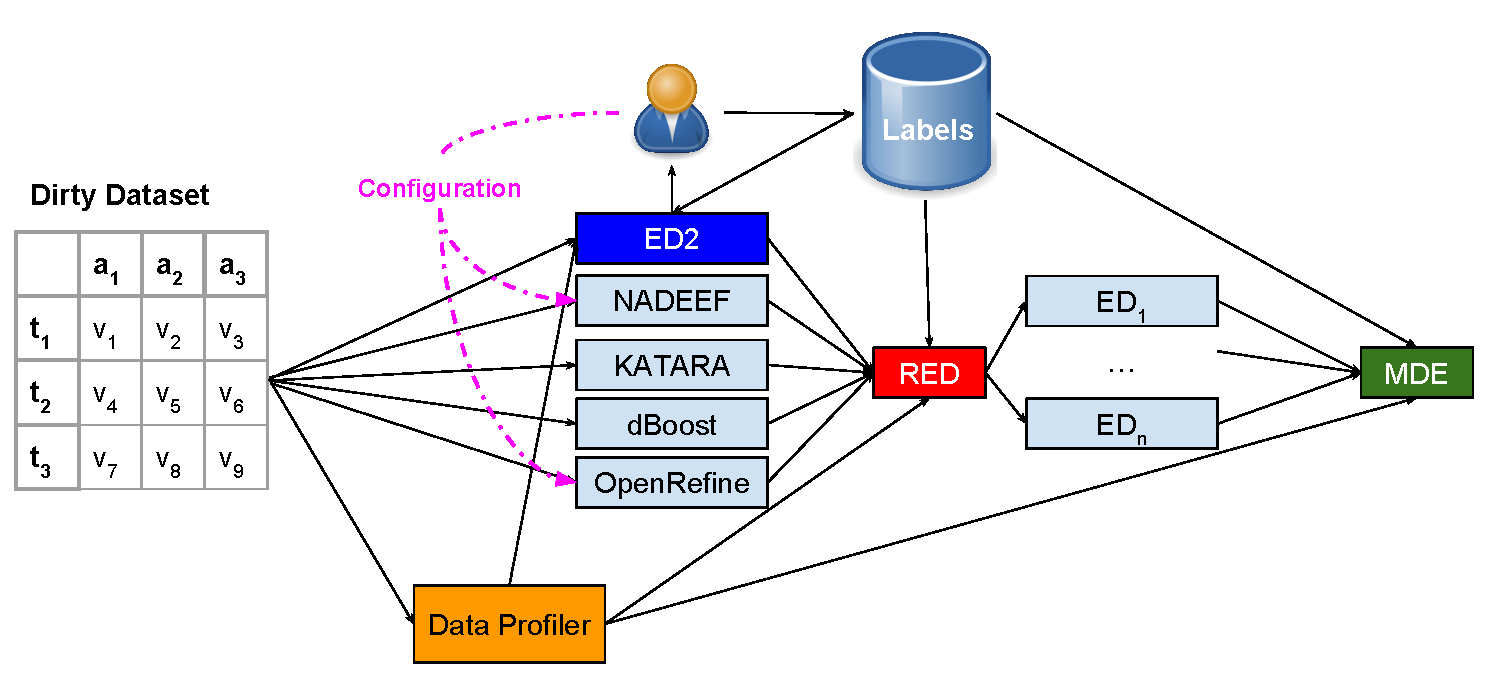
\includegraphics[width=0.9\textwidth]{img/demo.pdf}
	\caption{Architecture.}
	\label{figure:architecture}
\end{figure*}


\section{Conclusions}
\label{sec:conclusions}



\bibliographystyle{IEEEtran}

\bibliography{library/abbreviations,library/sigproc}

\end{document}
